\documentclass[aspectratio=169]{beamer}
\usefonttheme[onlymath]{serif}

\usepackage[utf8]{inputenc}
\usepackage{graphicx} % Allows including images
\usepackage{booktabs} % Allows the use of \toprule, \midrule and \bottomrule in tables
\usepackage{subfigure}
\usepackage{subfiles}
\usepackage{url}
\usepackage{amssymb}
\usepackage{amsmath}
\usepackage{xcolor,colortbl}
\usepackage[backend=bibtex,sorting=none]{biblatex}
\usepackage[AutoFakeBold, AutoFakeSlant]{xeCJK}

\addbibresource{reference.bib} 

\definecolor{NJUPurple}{rgb}{0.41568, 0, 0.37255} 
\colorlet{LightNJUPurple}{white!60!NJUPurple}
\colorlet{SuperLightNJUPurple}{white!90!NJUPurple}

\usecolortheme[named=NJUPurple]{structure}

%Information to be included in the title page:
\title{深度强化学习中的探索综述}
\author{\href{mailto:}{田鸿龙}}
\institute{Software Institute, Nanjing University}
\date{\today}


%Logo in every slide
\logo{%
  \makebox[0.98\paperwidth]{
    \href{https://www.nju.edu.cn}{
\includegraphics[height=0.75cm,keepaspectratio]{logos/nju_logo.jpg}}
    \hfill%
    \href{https://software.nju.edu.cn}{
\includegraphics[height=0.75cm,keepaspectratio]{logos/SE_logo.png}}%
  }
}

\setbeamertemplate{blocks}[rounded][shadow=true]
\setbeamercolor{block title}{fg=white,bg=LightNJUPurple}
\setbeamercolor{block body}{fg=black,bg=SuperLightNJUPurple}
\setbeamerfont{title}{shape=\bfseries,size=\Large}
\setbeamerfont{author}{shape=\bfseries}

\makeatletter
\setbeamertemplate{title page}{%
  \vbox{}
  \vfill
  \vskip2cm%<- added
  \begingroup
    \centering
    \begin{beamercolorbox}[sep=8pt,center]{title}
      \usebeamerfont{title}\inserttitle\par%
      \ifx\insertsubtitle\@empty%
      \else%
        \vskip0.25em%
        {\usebeamerfont{subtitle}\usebeamercolor[fg]{subtitle}\insertsubtitle\par}%
      \fi%     
    \end{beamercolorbox}%
    \vskip1em\par
    \vfill%<- added
    \begin{beamercolorbox}[sep=8pt,center]{author}
      \usebeamerfont{author}\insertauthor
    \end{beamercolorbox}
    \vskip-0.2cm%<- changed
    \begin{beamercolorbox}[sep=8pt,center]{institute}
      \usebeamerfont{institute}\insertinstitute
    \end{beamercolorbox}
    \vfill%<- added
    \begin{beamercolorbox}[sep=8pt,center]{date}
      \usebeamerfont{date}\insertdate
    \end{beamercolorbox}%
    \vskip0.5cm%<- changed
  \endgroup
%  \vfill%<- removed
}
\makeatother


\AtBeginSection[]
{
  \begin{frame}
    \frametitle{Table of Contents}
  \tableofcontents[
        currentsection,
        currentsubsection,
        subsectionstyle=show/show/hide,
        sectionstyle=show/shaded
    ]
  \end{frame}
}

% you can comment to disable TOC before every subsection
\AtBeginSubsection[]
{
  \begin{frame}
    \frametitle{Table of Contents}
  \tableofcontents[
        currentsection,
        currentsubsection,
        sectionstyle=show/shaded,
        subsectionstyle=show/shaded/hide,
    ]
  \end{frame}
}
% shape, colour of item, nested item bullets in itemize only
\setbeamertemplate{itemize item}[circle] \setbeamercolor{itemize item}{fg=NJUPurple}
\setbeamertemplate{itemize subitem}[circle] \setbeamercolor{itemize subitem}{fg=LightNJUPurple}
\setbeamertemplate{itemize subsubitem}[circle] \setbeamercolor{itemize subsubitem}{fg=SuperLightNJUPurple}
% font size of nested and nested-within-nested bulltes in both itemize and enumerate
% options are \tiny, \small, \scriptsize, \normalsize, \footnotesize, \large, \Large, \LARGE, \huge and \Huge


\setbeamerfont{itemize/enumerate subbody}{size=\scriptsize} 
\setbeamerfont{itemize/enumerate subsubbody}{size=\scriptsize}


\newenvironment{splitframe}[5]
%[1] ==> 1 parameter passed through {}
%[2] ==> 2 parameters passed through {}{}
%[4] ==> 4 parameters passed through {}{}{}{}
    {
    \begin{frame}{#3}
    \begin{columns}
    \column{#1\linewidth}
    \centering
    #4
    \column{#2\linewidth}
    \centering
    #5
    \end{columns}
    \centering
    \vspace{\baselineskip} % adds one line space
    }
    %Inside the first pair of braces (ABOVE) is set what your new environment will do before the text within, then inside the second pair of braces (BELOW) declare what your new environment will do after the text. Note second pair can be empty braces too.
    {
    \end{frame}
    }

\begin{document}

\frame{\titlepage}

\section{概述}

\subsection{传统强化学习中的探索问题}
\begin{frame}
  \frametitle{Bandit}
  \begin{figure}
    \centering
    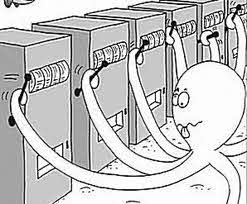
\includegraphics[width=0.2\textwidth]{imgs/bandit.jpeg}
  \end{figure}
  MAB问题:你进了一家赌场,假设面前有$K$台老虎机(arms)。我们知道,老虎机本质上就是个运气游戏,我们假设每台老虎机$i$都有一定概率$p_i$吐出一块钱,或者不吐钱( 概率 $i-p_i$)。假设你手上只有$T$枚代币(tokens),而每摇一次老虎机都需要花费一枚代币,也就是说你一共只能摇$T$次,那么如何做才能使得期望回报(expected reward)最大呢?
\end{frame}

\begin{frame}
  \frametitle{Expore or Exploit?}

  

  

\end{frame}

\subsection{深度强化学习}

\begin{frame}
  \frametitle{深度强化学习主流算法}

  \begin{figure}
    \centering
    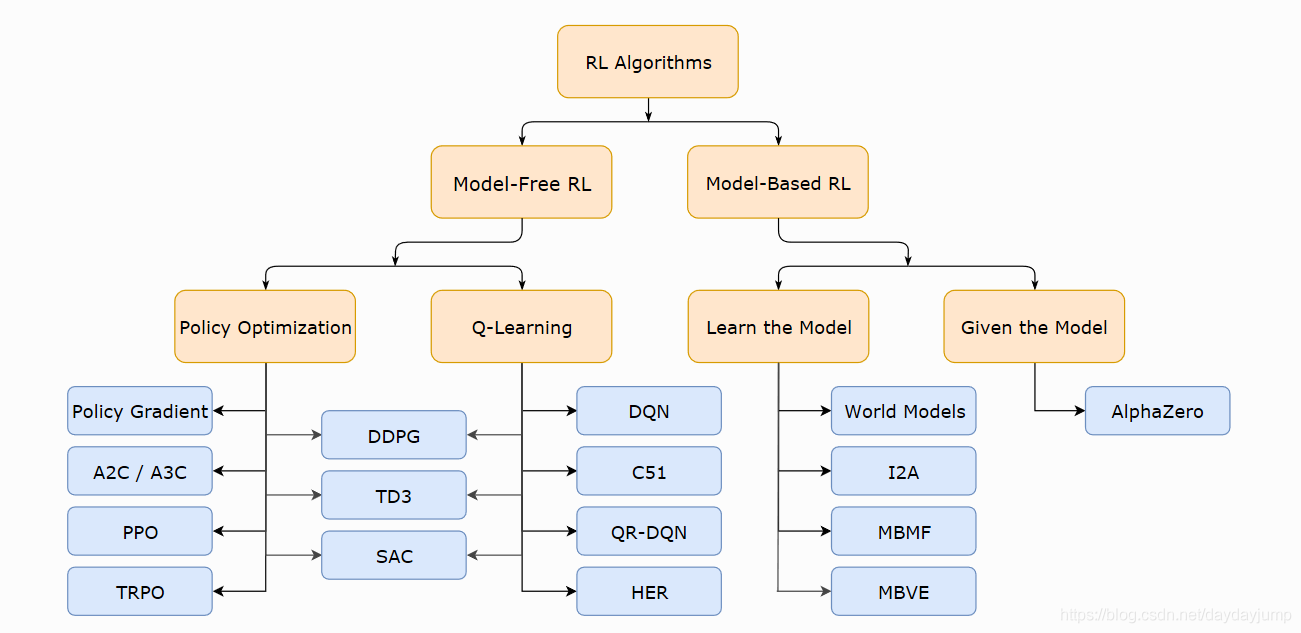
\includegraphics[width=0.8\textwidth]{imgs/DRL_agorithm.png}
  \end{figure}
\end{frame}

\begin{frame}
  \frametitle{两种思想}
  \begin{itemize}
    \item Value-Based:和传统强化学习一样,试图学到一个值函数(Q Function或者V Function),通过这个值函数贪心(或在贪心的基础之上探索)形成策略,理论基础是广义策略迭代。
    \item Policy-Based:基于函数逼近的方法,因为深度学习强大的拟合能力而成为深度强化学习的主流方法,直接学习$\pi:S \rightarrow A$,理论基础是策略梯度定理。
    \item 两种思想结合形成一大类Actor-Critic方法。其中A2C,A3C,PPO,TRPO等方法是On-Policy的,也被视为Policy-Based,而DDPG,TD3,D4PG,SAC等算法是Off-Policy的。
  \end{itemize}
\end{frame}

\begin{frame}
  \frametitle{Value-Based}
  \begin{itemize}
    \item DQN\cite{mnih2015human}是深度学习和强化学习结合的第一步,将Q-learning\cite{watkins1992q}和神经网络结合起来。
    \item DRQN\cite{hausknecht2015deep}将DQN和RNN结合起来,用来解决POMDP问题(但是因为训练成本和采样效率的问题,时序模型在强化学习中并不常见)。
    \item Dueling DQN\cite{wang2016dueling}将Q Funtion拆开分成Advantage Funtion和Value Funtion的和,提升了DQN的泛化性能。
    \item Double DQN\cite{van2015deep}结合Double Q-learning\cite{hasselt2010double}的思想,有效的缓解了值函数低估的问题。
    \item PER\cite{schaul2015prioritized}在DQN的基础上加入优先经验回放,进一步提升了采样效率。
    \item Distributional DQN\cite{dabney2017distributional}\cite{dabney2018implicit}\cite{bellemare2017distributional}将值函数扩展到值概率分布,进一步提升函数估计的准确性。
    \item Rainbow\cite{hessel2017rainbow}将上述方法结合,形成了有效的算法。
  \end{itemize}
\end{frame}

\begin{frame}
  \frametitle{Policy-Based}
  \begin{itemize}
    \item 策略梯度定理\cite{sutton1999policy}给出了Policy Gradient算法的可行性和性能分析。
    \item \cite{kakade2001natural}说明了梯度下降的局限性,将自然梯度下降用于Policy的优化。
    \item A3C\cite{mnih2016asynchronous}使用异步并行缓解采样效率低下的问题。
    \item TRPO\cite{schulman2015trust}结合\cite{kakade2001natural}给Policy Gradient的局部Off-Policy做出了理论分析。
    \item PPO\cite{schulman2017proximal}在\cite{schulman2015trust}的基础之上做了近似估计。
  \end{itemize}
\end{frame}

\begin{frame}[allowframebreaks]
\frametitle{References}
\printbibliography
\end{frame}

\end{document}

\end{document}